\section{EvoSuite}
EvoSuite is an example of an evolutionary algorithm that optimizes the whole test suite towards just one coverage criterion, rather than generating test cases directed towards multiple coverage criteria.
With EvoSuite, any collateral coverage isn't a concern since all coverage is intentional, given that the ultimate goal is to generate the whole test suite.
The algorithm starts with a randomly generated population of test suites.
The fitness function rewards better coverage of the source code; if two suites have the same coverage, the one with fewer statements is chosen. For each test suite, its fitness is measured by executing all of its test cases and keeping track of the executed methods and of the minimal branch distance for each branch.

\textbf{Expand on bloat in EvoSuite}





\section{NSGA-II}
A popular algorithm for many-objective search problems is the Non-dominated Sorting Genetic Algorithm II (NSGA-II). This algorithm is based on three principles:

\begin{itemize}
    \item It uses elitism when evolving the population: the most fit individuals are carried over along the offsprings.
    \item It uses an explicit diversity-preserving mechanism, the Crowding distance.
    \item It emphasizes the non-dominated solutions, as its name suggests.
\end{itemize}

First of all, in the context of test cases, domination can be expressed by the following relation:
\begin{figure}[!h]
    \centering
    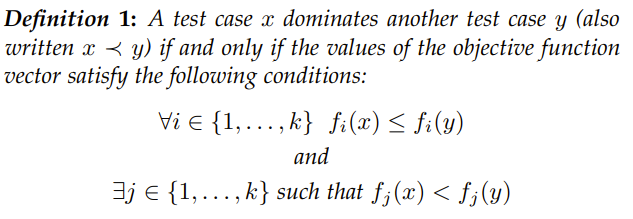
\includegraphics[scale=0.4]{./figures/test_Case_domination.PNG}
    \caption{Test case domination}
    \label{fig:test case domination}
\end{figure}


The NSGA-II algorithm works as follows:
\begin{itemize}
    \item Starting from an initial population of individuals Pt, generate an offspring population Qt of equal size and merge the two together, obtaining the population Rt.
    \item Perform non-dominated sorting of the individuals in Rt based on target indicators and classify them by fronts, i.e. they are sorted according to an ascending level of non-domination.  This ensures that the top Pareto-optimal individuals will survive to the next generation.
    \item If one of the fronts in the sorted sequence doesn't fit in terms of population size, crowding distance sorting is performed.
    \item Create the new population based on crowded tournament selection, then perform crossover and mutation. 
\end{itemize}


Figure 2.2 summarizes the main loop of the algorithm:
\begin{figure}[!h]
    \centering
    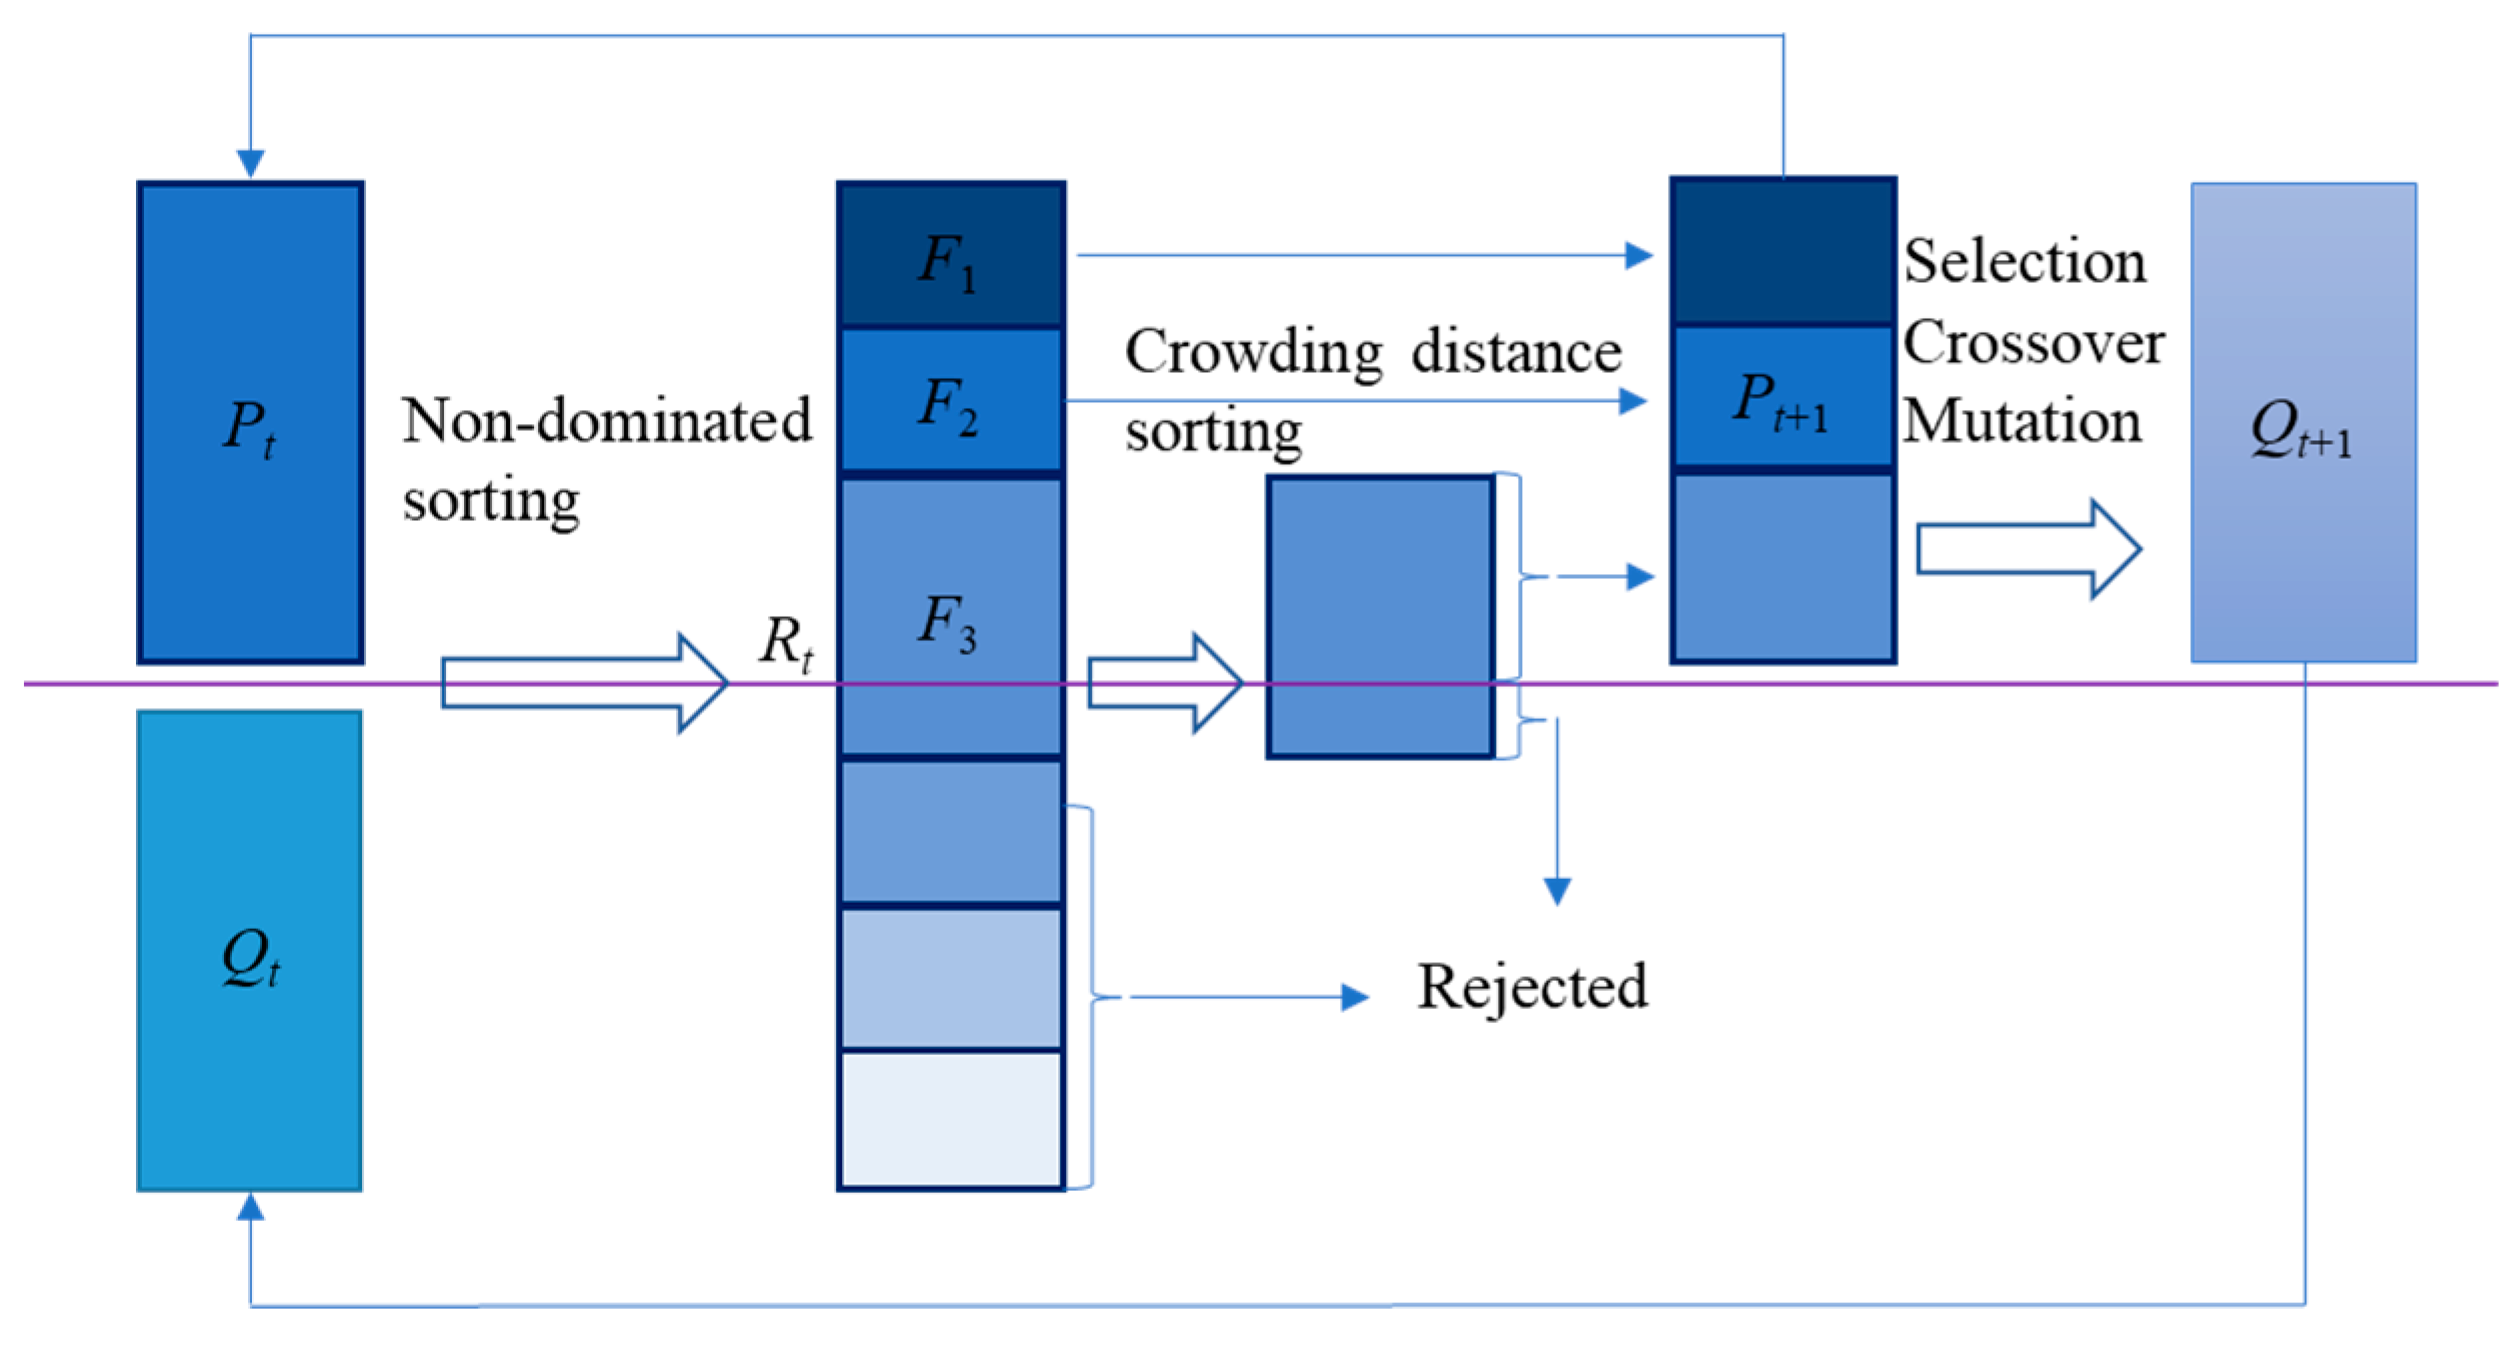
\includegraphics[scale=0.1]{./figures/nsga-ii.png}
    \caption{NSGA-II algorithm main loop}
    \label{fig:NSGA-II algorithm main loop}
\end{figure}


In the context of software engineering, NSGA-II has been applied to problems such as software refactoring and test case prioritization,
with two or three objectives. If the number of objectives begins to grow, however, the performance of the algorithm doesn't scale up well \cite{DBLP:journals/csur/LiLTY15}.
To overcome these limitations, there have been various adjustments and optimization of this algorithm...





\section{SPEA2}
Strength Pareto Evolutionary Algorithm (SPEA2)
Similarly to NSGA-II, SPEA2 isn't suitable for problems with more than three objectives. []




\section{MOSA}
MOSA \cite{DBLP:conf/icst/PanichellaKT15} is a GA proposed as an improvement over NSGA-II and SPEA2 for many-objective test case generation. With this algorithm, coverage of the different branches makes up the set of objectives to be optimized

As the first step, MOSA starts from a randomly generated initial population of test cases. 
To create the next generation, MOSA generates offsprings by implementing the classic operations of selection, crossover and mutation. 
Before selection occurs however, for each uncovered branch, the test case with the lowest objective score(branch distance + approach level) is determined; these test cases will have assigned the rank 0 and will make up the first front. The remainder of the test cases will be sorted according to the traditional NSGA-II approach.

After the rank assignment step is complete, the crowding distance is calculated to determine which individuals to select: the individuals with higher distance from the rest are given a higher chance of being selected. The algorithm attempts to select as many test cases as possible, starting from front 0,  until the population size is reached

Finally, MOSA uses an archive population that keeps track of the best performing test cases, in order to form the final test suite.


\section{DynaMOSA}
DynaMOSA, Dynamic Many-Objective Sorting Algorithm \cite{DBLP:journals/tse/PanichellaKT18} is an approach that focuses on ..., and has been developed as an evolution of MOSA. This latter solution implements a many-objective GA to tackle test case generation and has three main features: 
\begin{itemize}
    \item instead of ranking candidates for selection based on their Pareto optimality, it uses a preference criterion. This criterion selects the test case with the lowest objective score for each uncovered target; these selected individuals are given a higher chance of survival, while other test cases are ranked with the traditional NSGA-II approach.
    \item The search is focused only on the uncovered coverage targets.
    \item All tests that satisfy one or more of the uncovered targets will be archived and used as the final test suite once the search ends.
\end{itemize}

In many-objective optimization problems, candidate solutions are typically evaluated in terms of Pareto dominance and Pareto optimality.

DynaMOSA has been employed with Java classes.





\section{OCELOT}
Optimal Coverage sEarch-based tooL for sOftware Testing, OCELOT \cite{DBLP:conf/ssbse/ScalabrinoGNOL16} is a test case generation tool for C programs that implements both a multi-target approach based on MOSA, and new iterative single-target appproach named LIPS, Linear Independent Path-based Search.

Tested with MOSA but not with DynaMOSA.